\subsection{RandSVD}
\makesubcontentsslidessec


\begin{frame}[fragile]
\fontsize{8pt}{10}\selectfont
\begin{block}{Randomized SVD\footnotemark}
  \begin{minipage}{.55\textwidth}
    \begin{center}
      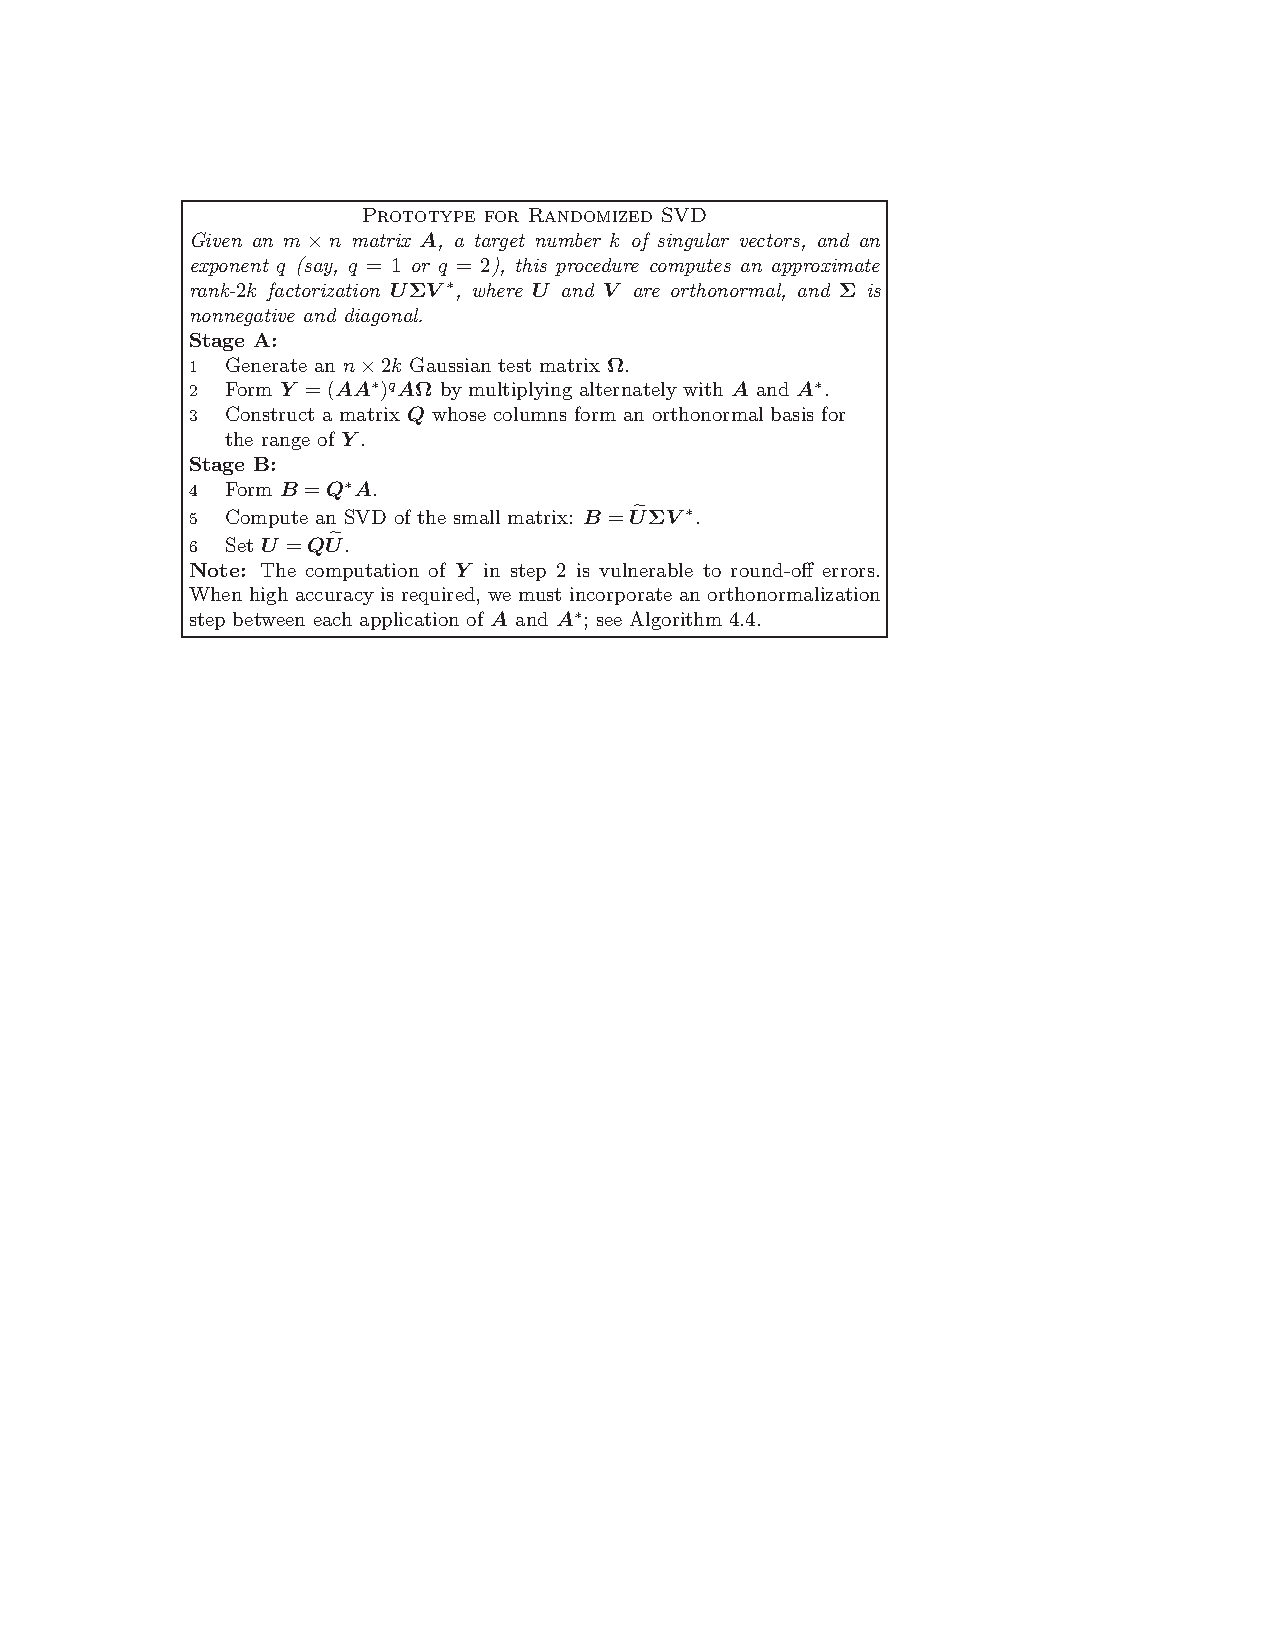
\includegraphics[height=.55\textheight]{../common/pics/randsvd/randSVDalg}
      \\
      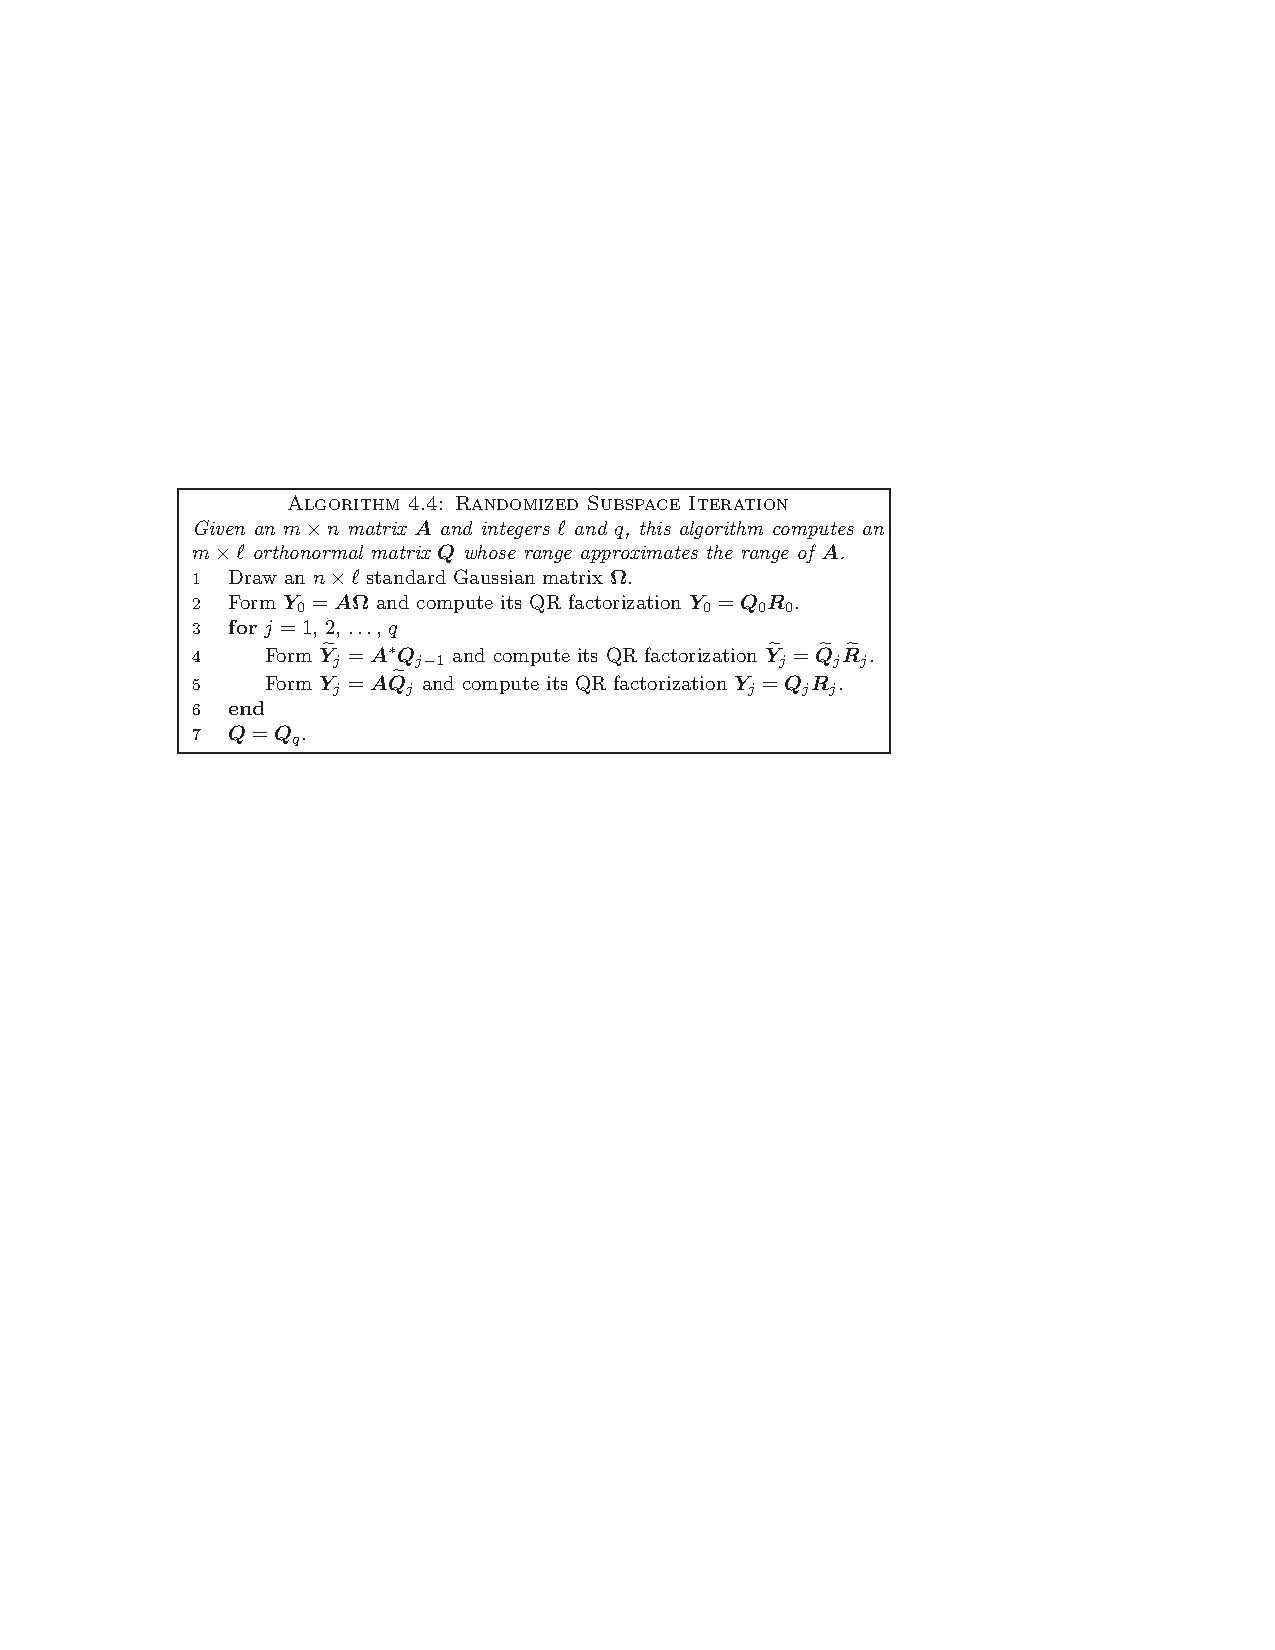
\includegraphics[height=.35\textheight]{../common/pics/randsvd/randSVDalg4_4}
    \end{center}
  \end{minipage}
%   \hspace{.01cm}
  \begin{minipage}{0.430\textwidth}
\begin{lstlisting}[title=Serial 
R,basicstyle=\tiny,backgroundcolor=\color{grayish} 
,numberstyle=\tiny\color{black},keywordstyle=\color{black},commentstyle=\color{ 
dkgreen},stringstyle=\color{black},escapeinside={(*@}{@*)}]
randSVD <- function(A, k, q=3)
  {
    ## Stage A
    Omega <- (*@ matrix(rnorm(n*2*k),@*) (*@ nrow=n, ncol=2*k) @*)
    Y <- A %*% Omega
    Q <- qr.Q(qr(Y))
    At <- t(A)
    for(i in 1:q)
      {
        Y <- At %*% Q
        Q <- qr.Q(qr(Y))
        Y <- A %*% Q
        Q <- qr.Q(qr(Y))
      }
    
    ## Stage B
    B <- t(Q) %*% A
    U <- La.svd(B)$u
    U <- Q %*% U
    U[, 1:k]
  }
\end{lstlisting} %balance$
\end{minipage}
{\fontsize{6pt}{10}\selectfont $^1$Halko N, Martinsson P-G 
  and Tropp J A 2011 Finding structure with randomness: probabilistic 
algorithms 
  for constructing approximate matrix decompositions \emph{SIAM Rev.} 
\textbf{53} 
  217--88}
\end{block}
\end{frame}


\begin{frame}[fragile]
 \fontsize{8pt}{10}\selectfont
\begin{block}{Randomized SVD}
  \hfill
  \begin{minipage}{0.430\textwidth}
\begin{lstlisting}[title=Serial 
R,basicstyle=\tiny,backgroundcolor=\color{grayish} 
,numberstyle=\tiny\color{black},keywordstyle=\color{black},commentstyle=\color{ 
dkgreen},stringstyle=\color{black},escapeinside={(*@}{@*)}]
randSVD <- function(A, k, q=3)
  {
    ## Stage A
    Omega <- (*@ \textcolor{blue}{matrix(rnorm(n*2*k),} @*)(*@ \textcolor{blue}{ nrow=n, ncol=2*k)} @*)
    Y <- A %*% Omega
    Q <- qr.Q(qr(Y))
    At <- t(A)
    for(i in 1:q)
      {
        Y <- At %*% Q
        Q <- qr.Q(qr(Y))
        Y <- A %*% Q
        Q <- qr.Q(qr(Y))
      }
    
    ## Stage B
    B <- t(Q) %*% A
    U <- La.svd(B)$u
    U <- Q %*% U
    U[, 1:k]
  }
\end{lstlisting} %balance$
  \end{minipage}
  \hfill
  \begin{minipage}{0.430\textwidth}
\begin{lstlisting}[title=Parallel pbdR,basicstyle=\tiny,backgroundcolor=\color{
grayish}, numberstyle=\tiny\color{black},keywordstyle=\color{black},
commentstyle=\color{dkgreen},stringstyle=\color{black},escapeinside={(*@}{@*)}]
randSVD <- function(A, k, q=3)
  {
    ## Stage A
    Omega <- (*@ \textcolor{blue}{ddmatrix("rnorm",} @*)(*@ \textcolor{blue}{nrow=n, ncol=2*k)} @*)
    Y <- A %*% Omega
    Q <- qr.Q(qr(Y))
    At <- t(A)      
    for(i in 1:q)
      {
        Y <- At %*% Q   
        Q <- qr.Q(qr(Y))
        Y <- A %*% Q    
        Q <- qr.Q(qr(Y))
      }
    
    ## Stage B
    B <- t(Q) %*% A     
    U <- La.svd(B)$u 
    U <- Q %*% U     
    U[, 1:k]
  }
\end{lstlisting}  % balancing $
  \end{minipage}
\hfill
\end{block}
\end{frame}

\begin{frame}
  \begin{block}{Randomized SVD}
    \begin{center}
      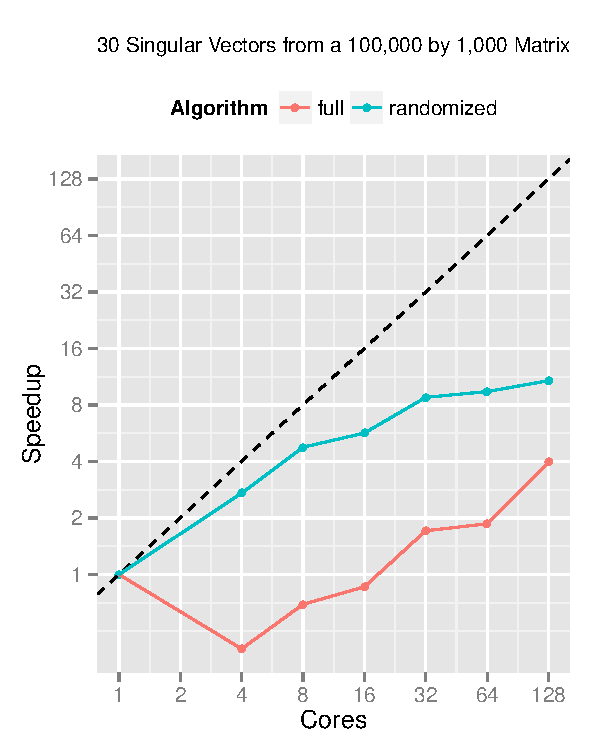
\includegraphics[width=.4\textwidth]{../common/pics/randsvd/randSVDspeedup}
      \hspace{1cm}
      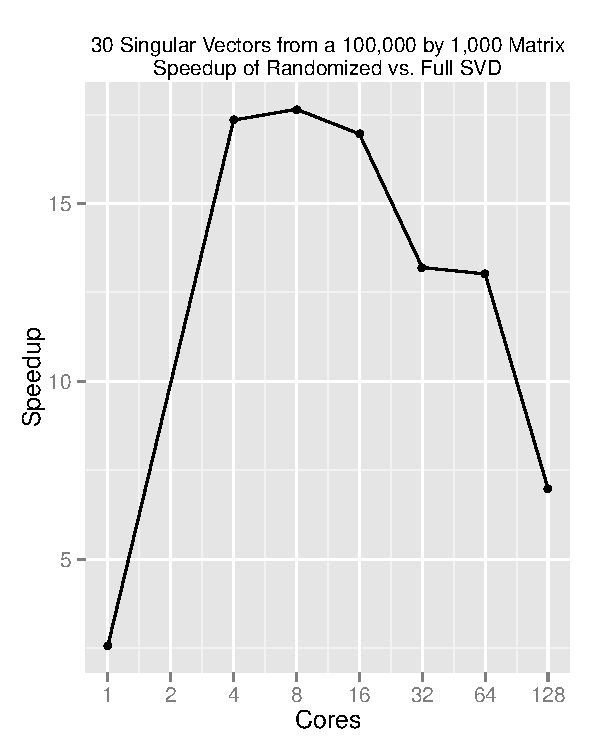
\includegraphics[width=.4\textwidth]{../common/pics/randsvd/randSpeedupSVD}
    \end{center}
  \end{block}
\end{frame}